\begin{figure}[ht]
\centering
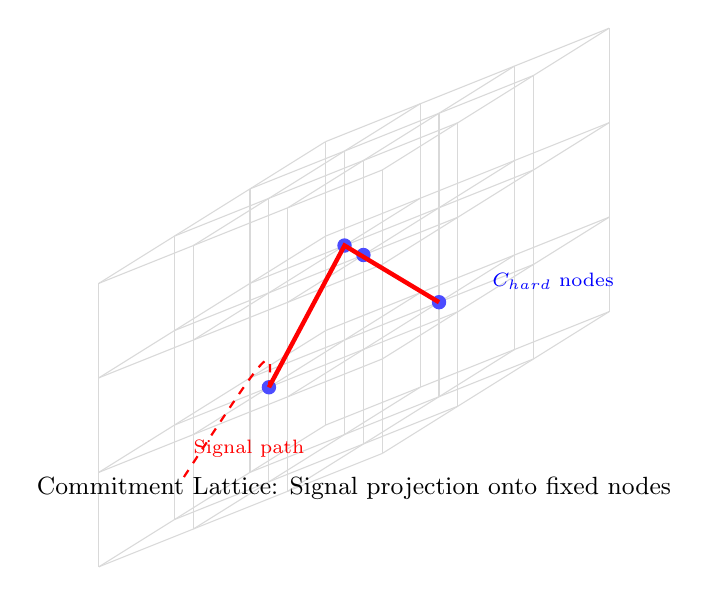
\begin{tikzpicture}[scale=1.2, x={(1cm,0.4cm)}, y={(0.8cm,0.5cm)}, z={(0cm,1cm)}]
    % Draw the 3D Lattice Grid
    \foreach \x in {0,1,2,3}
        \foreach \y in {0,1,2,3}
            \draw[gray!30, thin] (\x, \y, 0) -- (\x, \y, 3);
    \foreach \x in {0,1,2,3}
        \foreach \z in {0,1,2,3}
            \draw[gray!30, thin] (\x, 0, \z) -- (\x, 3, \z);
    \foreach \y in {0,1,2,3}
        \foreach \z in {0,1,2,3}
            \draw[gray!30, thin] (0, \y, \z) -- (3, \y, \z);

    % Draw the "Hard Commitment Nodes"
    \foreach \x/\y/\z in {1/1/1, 1/2/2, 2/1/2, 2/2/1}
        \filldraw[blue!70] (\x, \y, \z) circle (2pt);

    % Draw the Signal Path being "Projected" to the Lattice
    \draw[red, thick, dashed] (0.5, 0.5, 0.5) .. controls (1.2, 0.8, 1.5) .. (1, 1, 1);
    \draw[red, ultra thick] (1,1,1) -- (1,2,2) -- (2,2,1);
    
    % Labels
    \node[anchor=north, font=\small] at (1.5, 1.5, -0.3) {Commitment Lattice: Signal projection onto fixed nodes};
    \node[anchor=west, font=\scriptsize, text=blue] at (2.3, 2.2, 1) {$C_{hard}$ nodes};
    \node[anchor=west, font=\scriptsize, text=red] at (0.5, 0.5, 0.8) {Signal path};
\end{tikzpicture}
\caption{Three-dimensional commitment lattice structure. Blue nodes represent hard commitment vertices ($C_{hard}$) that serve as fixed points in the signal space. The red path shows how a signal (dashed: original trajectory) is projected onto the lattice structure (solid: enforced path), ensuring topological stability under transformation.}
\label{fig:commitment-lattice}
\end{figure}
